
\begin{document}
\pagestyle{empty}
\chapter{Experimental study of mutagenesis in \textit{C. elegans}}

\section{Introduction}

The first chapter of this thesis gave an overview of the 
current state of knowledge of endogenous and exogenous mutagenesis and 
its relation to cancer. Based on this vast amount of knowledge, I will 
try to expand the understanding of mutational signatures, their translatability 
across species, and their behaviour under different genetic conditions.

Mutational signatures have become a useful tool 
of oncological investigations, providing the means to uncover the functional causes 
of tumour development. Some of the computationally extracted 
signatures have been associated with the underlying processes, and a 
small fraction have been confirmed in experimental work. However several questions 
remain unclear: whether these associations are trustworthy and the relevant signatures 
are directly linked to the associated factor, what are the origins of other signatures, 
and how consistent is the signal across different organisms, tissues and genetic backgrounds.

In this chapter, I will introduce the mutagenesis screen performed
in \textit{C. elegans} and describe the bioinformatics pipeline to deliver 
the results from the sample stage to mutational spectra, creating the basis
for studying experimental signatures of different factors contributing
to mutagenesis.

%%%%%%%%%%%%%%%%%%%%%%%%%%%%%%%%%%%%%%%%%%%%%%%%%%%%%%%%%%%%%%%%%%%%

\subsection*{Contributions}

The experimental work on sample preparation was conducted at the University of Dundee by 
Bettina Meier and colleagues. DNA sequencing, read alignment and basic variant calling for 
base substitutions and insertions/deletions was done by the Sanger Institute facilities. 
Subsequent bioinformatics analyses such as filtering, classification and analyses of mutational 
load and distributions were performed by me.

\todo[inline]{Data and code availability}

%%%%%%%%%%%%%%%%%%%%%%%%%%%%%%%%%%%%%%%%%%%%%%%%%%%%%%%%%%%%%%%%%%%%
\section{Exploiting \textit{C.elegans} as an experimental system for mutagenesis study}

In this study we used \textit{C. elegans} as a model organism to present a systematic 
screen of genotoxin and DNA repair deficiency signatures, with the same setup as in 
\cite{Meier1}. Currently the dataset contains 3242 samples from 985 experiments with 
13 genotoxins under 90 different genetic conditions, including single and double 
knock-outs of DNA repair associated genes. 

\todo[inline]{self-fertilization!!!}

This organism is a suitable experimental model in many aspects: it is easy to manipulate, 
it has a well annotated genome (\cite{antoshechkin2007versatile}), its turnover time is short with a lifespan of 
approximately 3 days (\cite{hope1999c}). \textit{C. elegans} genome, while 
being relatively small (approximately 100 Mbps) and having an extremely low proportion 
of "junk DNA", contains a large number of orthologs of 
many human DNA repair associated genes (\cite{kaletta2006finding}). Moreover, it has a low
background mutation rate of about 0.2-0.5 mutations per genome per generation (\cite{denver2009genome}), 
which allows to detect even small changes in the rates of mutation acquisition.

Previously established \textit{C. elegans} mutation accumulation assays demonstrated 
that defects in major DNA damage response and DNA repair pathways, which included 
nucleotide excision repair, base excision repair, DNA crosslink repair, DNA end-joining 
and apoptosis did not lead to overtly increased mutation rates when lines were propagated 
for 20 generations (\cite{Meier2014-aa}). These studies were now extended to MMR deficiency 
conferred by MutL mutations. The experimental setup takes advantage of the 3-4 days 
life cycle of \textit{C. elegans} and its hermaphroditic reproduction of self-fertilization. 
This allows the propagation of clonal \textit{C. elegans} lines, which in each 
generation pass through a single cell bottleneck provided by the zygote. 

On the other hand, high fidelity of replication and smaller non-coding fraction of the genome 
limit the numbers of mutations which may be observed before the \textit{C.elegans} lineage 
becomes sterile or non-viable *REF*. In order to mimic the mutation accumulation in somatic 
cells necessary for cancer development, \textit{C. elegans} were introduced with DNA repair 
deficiencies and grown through several generations essentially being put through a single-cell 
bottleneck at each generation change.

\subsection{Data collection and filtering}

\subsubsection*{Study design}

The samples were coming from two types of experiments: mutation accumulation and mutagen exposure. 
In the first type, the genetic knock-outs of a DNA repair relevant genes are introduced, and the 
worm is further propagated for 20 or 40 generations. In the latter type, the worms of particular 
genetic backgrounds were exposed to certain cytotoxins, and their progeny was sent to sequencing 
to analyze the range of acquired mutations. When possible, the mutagenized worms were propagated 
for several generations, but in most cases already the first generation of progeny was sterile 
or lethally ill. \textit{C. elegans} mutants were obtained from the collaborating lab at the 
university of Dundee upon back-crossing and further propagation as described in \cite{Meier2014-aa} 
and \cite{Meier2018-qz}.

The schematic description of the experiments is depicted in Figure \ref{exp_types}. Wild-type 
and \textit{C. elegans} mutants of selected genes from 10 different DNA repair pathways 
were propagated over several generations or exposed to increasing doses of different 
classes of genotoxins. Genomic DNA was extracted from samples before and after 
accumulation without and with treatment and whole genome sequenced to determine 
mutational spectra. Mutations were classified into 119 mutation classes: 96 single 
base substitutions classified by change and ‘5 and 3’ base context, di- and 
multi-nucleotide variants (MNV), 6 types of deletions of different length and 
context, 2 types of complex indels, 6 types of insertions and 7 classes of structural variants.

\begin{figure}
  \centering
  \centerline{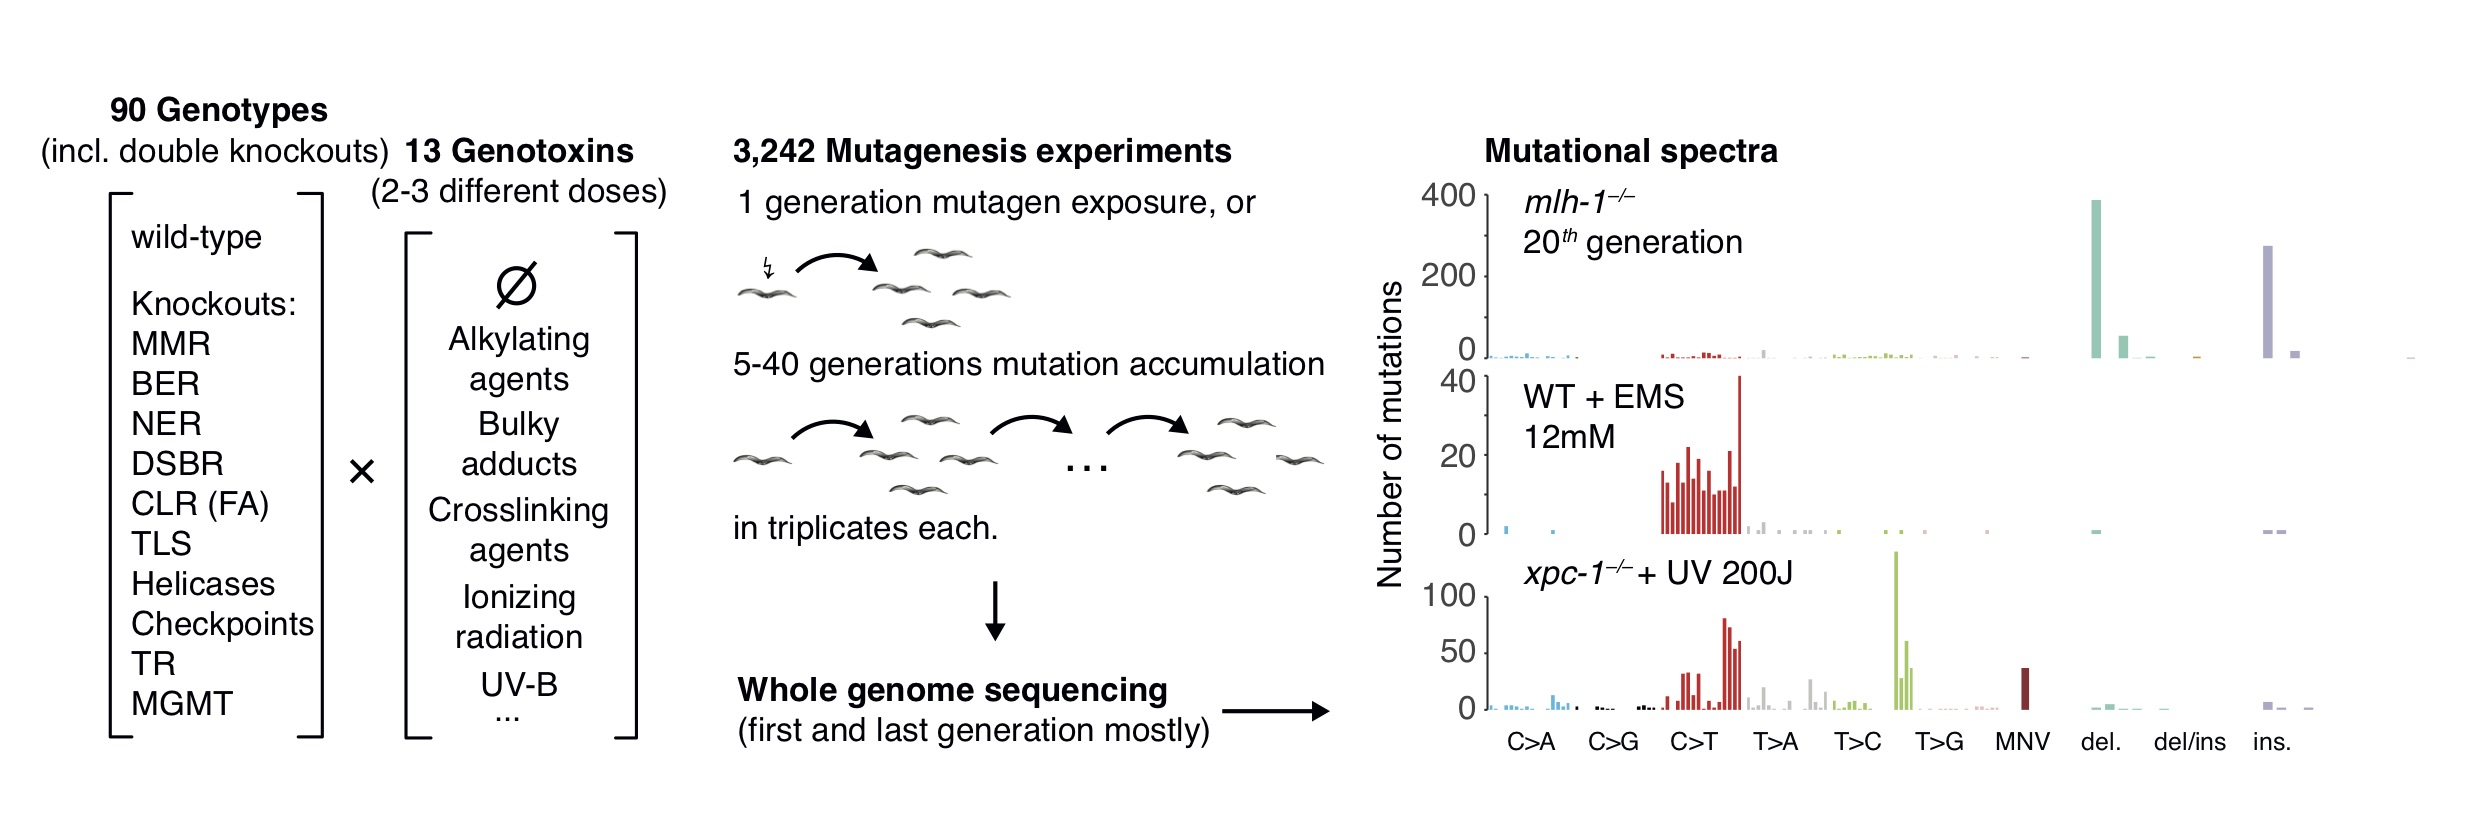
\includegraphics[width=1\textwidth]{figures/thesis_figure_worm_experiment.jpg}}
  \caption{Experimental design of the study.}
  \label{exp_types}
\end{figure}

Panel of substances used for mutagen exposure experiments consisted of substances and 
exposures employed in cancer treatments: 
alkylating agents (dimethyl sulfate (DMS), ethyl methanesulfonate (EMS), methyl 
methanesulfonate (MMS), mechlorethamine (Mech), hydroxyurea (HU)), irradiations 
(gamma-irradiation (IR), X-rays (Xray) and simulated UV-B irradiation (UV)), 
agent creating bulky adducts (aflatoxin-B1, aristolochic acid), crosslinking agents 
(cisplatin).

List of genetic knock-outs included genes representing all crucial DNA repair pathways: 
we consider 6 genes responsible for translesion synthesis (TLS), 13 backgrounds associated 
with single-strand break repair (SSBR) deficiency, 28 conditions associated with double-strand 
breaks repair (DSBR) deficiency, 6 helicases with different additional properties, 7 DNA damage 
checkpoint genes and 5 genes related to damage-caused apoptosis. Full list of genetic conditions with respective pathways and their effects on  genomic stability can be find in the Appendix.

\subsection{Overview of the data}

Here should be a tSNE plot of all samples coloured by mutagen or coloured by pathway.

%%%%%%%%%%%%%%%%%%%%%%%%%%%%%%%%%%%%%%%%%%%%%%%%%%%%%%%%%%%%%%%%%%%%%%%%%%%%%%%%

\section{Extracting mutational signatures from experimental data}

\textbf{Calculation of mutational patterns of individual factors in \textit{C. elegans} experiments}


\subsubsection*{Model}

To assess the individual contributions of every factor, we employed positive Poisson additive 
model with $r$ responses (reflecting the variant classes), that includes $k$ genetic, 
mutagenic, gene interaction and gene-mutagen interaction factors, for every response 
class $j$:

\[Y_{j} \sim Pois(\lambda_{j}), \lambda_{j} \in  \mathbb{R}_{+} , j = 1, ..., r\]

\begin{equation}
E[Y_j] = \lambda_j = X \beta_{j}^{T} = X_{gen} \beta_{j,gen}^T + X_{mut} \beta_{j,mut}^T + X_{int} \beta_{j,int}^T, \beta_j \in (\mathbb{R}_{+} \cup {0})^k
\end{equation}






For the assessment of the basic signatures created my DNA repair deficiencies and 
genotoxin exposures, we first used an additive Poisson model. For each sample, its 
full mutational profile (including 96 base substituion types, 2 categories of 
multinucleotide substitutions, 6 types of deletions, 2 types of complex indels, 
6 types of insertions and 7 types of structural variants) was modelled as

\[Y = \{Y_{j}\}_{j=1}^{119}, Y_{j} \sim Pois( \lambda_{j} ),\]

\[E[Y_{j}] = \lambda_{j} = N \cdot \left( \beta_{j,b} + X_{g_{1}} \cdot \beta_{j,g_{1}} + X_{g_{2}} \cdot \beta_{j,g_2} + X_{g_1:g_2} \cdot \beta_{j,g_{1}:g_{2}} ) \right),\]

\[beta_{j,\cdot} \ge 0,\]

where $Y_{j}$ is a number of particular mutations of type $j$, $N$ is the number 
of generations, $g1$ and $g2$ – gene knock-outs, $b$ - background contribution, 
and coefficient $X_{g} \in {0,1}$ indicates the presence of a particular factor.

To extract the model parameters, we further implemented non-negative matrix 
factorization with generalized Kullback-Leibler divergence minimization:

\[D(A||B) = \sum_{i,j} A_{ij} log(\frac{A_{ij}}{B_{ij}} ) - A_{ij} + B_{ij}\]

This approach is equivalent to maximum likelihood estimation in non-negative Poisson 
regression model in the case of fixed multiplier $X$: 

\[Y = X \beta, \beta \in M_{k \times r} (\mathbb{R}_{+} \cup {0})\]

\begin{equation}
\begin{split}
\ell(Y|X,\beta) &= \sum_{i,j} \left[Y_{ij}  log⁡(X \beta)_{ij} - (X \beta)_{ij} \right] + C \\
&= - \sum_{i,j} \left[Y_{ij}  log⁡ \left( \frac{Y_{ij}}{(X\beta)_{ij}} \right) - Y_{ij} + (X\beta)_{ij} \right] + \tilde{C} \\ 
&= - D(Y||X\beta) + \tilde{C}
\end{split}
\end{equation}

The update rule we used looks as follows:

\begin{equation}
\beta_{ij} \leftarrow \beta_{ij} \cdot \frac{\sum_s \frac{X_{si} Y_{sj}}{(X\beta)_{sj}}} {\sum_t X_{ti}}
\end{equation}

Coefficient matrix $\beta$ was update on every step till both the change in KL 
generalized distance \(D(Y||X\beta)\) and average change in the elements of $\beta$ 
reach the certain threshold. 

The variance and significance of the parameters calculated via NMF were estimated using 
Poisson maximum likelihood estimation and constrained Wald test (\cite{Molenberghs2007-xo}).

We calculated maximum likelihood estimates of all vectors $\beta_{j,\cdot}$ for every 
signature using an algorithm equivalent to non-negative matrix factorization with a 
fixed multiplier and KL-divergence as distance measure (\cite{Lee1999-at}, \cite{Cemgil2009-mh}). 
95\% confidence intervals for signatures were calculated as CIs for Poisson regression coefficients.

v
\textbf{Comparison of mutational signatures}

Similarity between the signatures was calculated via cosine similarity: 

\[similarity(S1,S2) = \frac{( <S_1, S_2> )}{( (\norm{S1}) \cdot (\norm{S2}) )},\]

where $<S1, S2>$ is a scalar product of signature vectors. The threshold for ‘high’ similarity was taken as 0.80, as the similarity assessment within COSMIC cancer signature set showed that only 3.4\% of pairs have cosine similarity above this threshold, and also it is the 95\% quantile for similarity distribution between random uniformly generated ‘mutational profile’ vectors from positive cone (Appendix 2).

%%%%%%%%%%%%%%%%%%%%%%%%%%%%%%%%%%%%%%%%%%%%%%%%%%%%%%%%%%%%%%%%%%%%

\section{Translation of mutational signatures between species}

\subsection{Genomic differences}

Different genome size and coding fraction

In order to make the comparison between \textit{C. elegans} and human mutational signatures valid,
the experimental signatures acquired from \textit{C. elegans} were adjusted to the human exome or genome trinucleotide
frequencies. The probabilities for 96 base substitutions were multiplied by the ratio of respective 
trinucleotide counts observed in the human exome (hg19, the counts pre-calculated in \cite{Rosenthal})
to those in the \textit{C. elegans} reference genome (Figure \ref{Trinucleotide}).

\begin{figure}[h]
  \centering
  \centerline{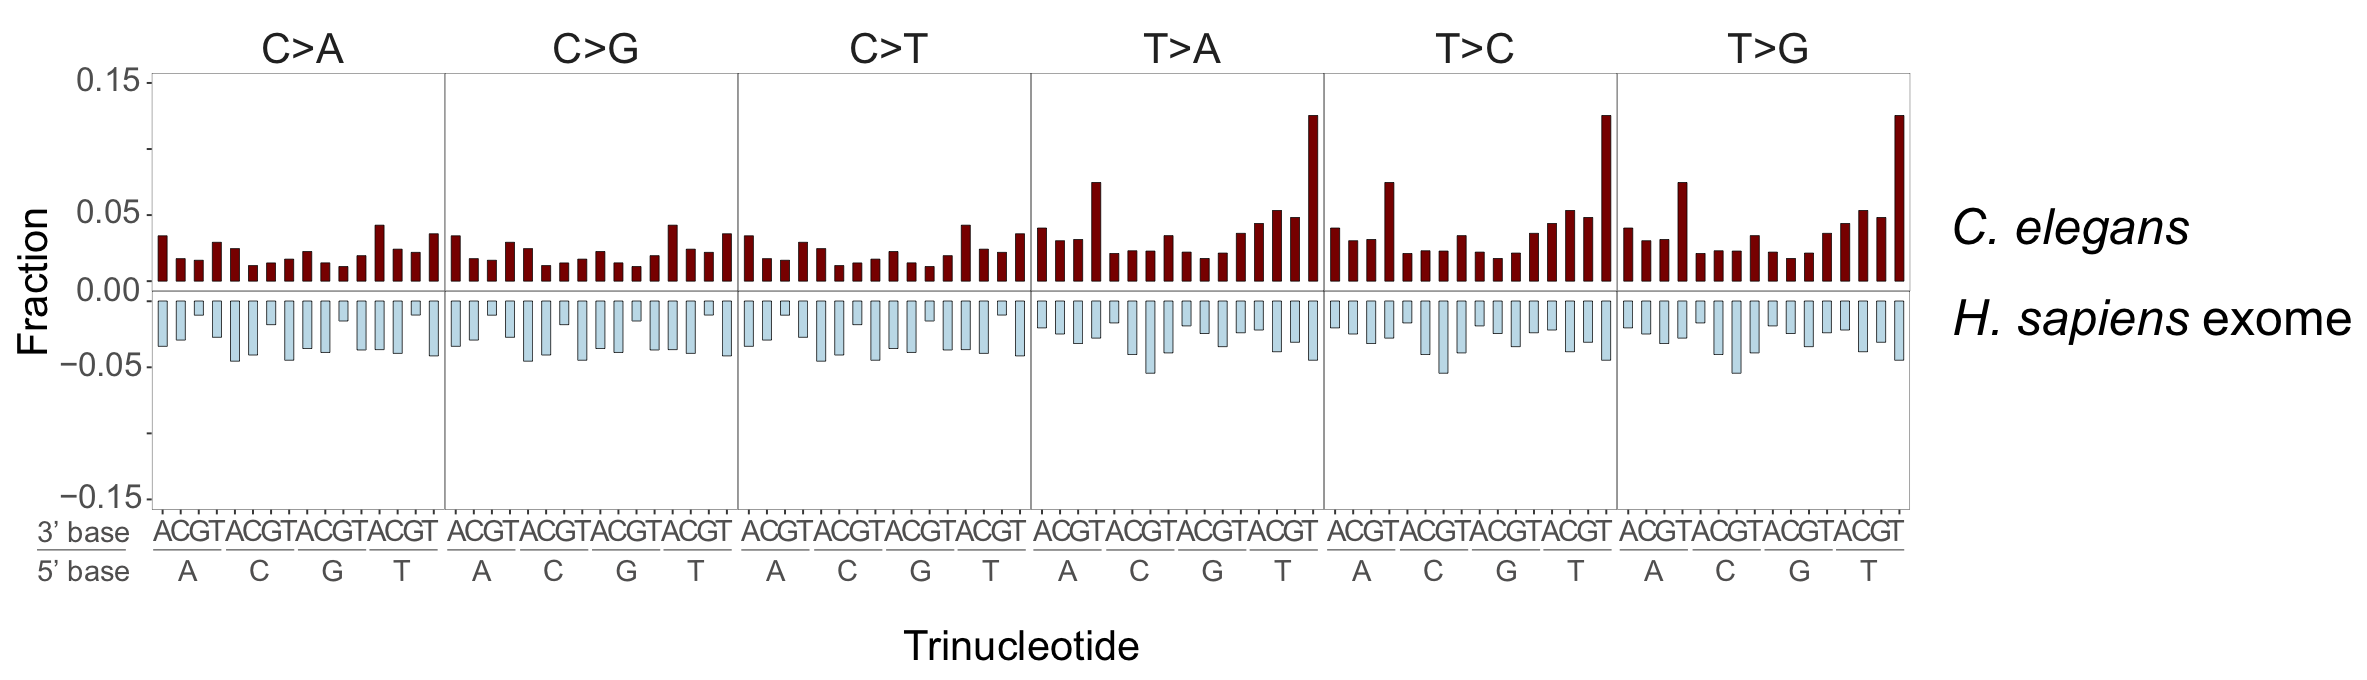
\includegraphics[width=1\textwidth]{figures/Trinucleotide.png}}
  \caption{Trinucleotide context comparison between \textit{C. elegans} genome and \textit{H. sapiens} exome.}
  \label{Trinucleotide}
\end{figure}

\section{Discussion}


\end{document}